%% LyX 1.3 created this file.  For more info, see http://www.lyx.org/.
%% Do not edit unless you really know what you are doing.
\documentclass[11pt,a4paper]{article}
\usepackage[T1]{fontenc}
\usepackage[latin1]{inputenc}
\usepackage[italian]{babel}
\usepackage{graphicx}

\makeatletter

%%%%%%%%%%%%%%%%%%%%%%%%%%%%%% LyX specific LaTeX commands.
%% Bold symbol macro for standard LaTeX users
\newcommand{\boldsymbol}[1]{\mbox{\boldmath $#1$}}


%%%%%%%%%%%%%%%%%%%%%%%%%%%%%% User specified LaTeX commands.
\usepackage{verbatim}
\usepackage{babel}
\makeatother
\begin{document}

\title{Calcolo dei fattori di franck condon su biatomiche}

\maketitle
Valuteremo i fattori di franck condon per alcuni casi ideali su una
molecola semplice, l'acido fluoridrico. Il programma dalton fornisce
l'output necessario per il programma lifetime di toniolo, tuttavia
\`e necessario convertire i dati, dal momento che lifetime pretende
l'input come dal programma venus. Lifetime, per il calcolo dei fcf,
necessita di:

\begin{enumerate}
\item geometria della molecola negli stati fondamentale ed eccitato
\item modi normali di vibrazione e relative frequenze per lo stato fondamentale
ed eccitato.
\end{enumerate}
Queste informazioni vanno poste nei file08 e file07 rispettivamente.
Notare che la routine di toniolo vuole anche la matrice delle derivate
delle coordinate interne rispetto alle coordinate normali, ma attraverso
una direttiva di preprocessore non viene compilata, dal momento che
non \`e necessaria per il calcolo dei fcf. Il formato di questa parte
del file di input \`e il seguente, per un esempio del CH3NO
\begin{footnotesize}
\begin{verbatim}
1)      EQUILIBRIUM COORDINATES IN THE P.A. SYSTEM AND ATOMIC MASSES
2)    1.9858403578   -0.4898557694   0.0000000000    29165.1225068910
3)    0.2275802019    1.0026037055   0.0000000000    25532.6525630505
4)   -2.2129773571   -0.3505195052   0.0000000000    21894.9892098308
5)   -3.2478112579    0.1999055914   1.7029005918     1837.4169364646
6)   -3.2478112579    0.1999055914  -1.7029005918     1837.4169364646
7)   -1.8176175996   -2.3796600066   0.0000000000     1837.4169364646
\end{verbatim}
\end{footnotesize}

Prima della parentesi il numero di linea, da non specificare. Importante notare
che 
\begin{enumerate}
\item \`e necessario specificare la scrittura in riga 1
\item le coordinate vanno date in bohr, le masse in unit\`a atomiche 
\item il formato \`e libero
\end{enumerate}
per i modi normali di vibrazione, occorre specificare 

\begin{enumerate}
\item la frequenza di ogni modo normale di vibrazione, \textbf{inclusi} i modi
traslazionali e vibrazionali
\item la matrice L le cui righe rappresentano le combinazioni lineari di
coordinate cartesiane che forniscono le coordinate normali. Questa matrice
viene gestita e presentata dai vari programmi con i vettori ordinati per
colonne. Essendo la matrice unitaria, tale matrice per colonne \`e denominata
$L^{-1}$
\end{enumerate}
Il formato \`e decisamente pi\`u complesso. occorre specificare alcune
righe pi\`u o meno vuote. L'ordine degli autovalori \`e importante.
Vanno ordinati dai modi con frequenza pi\`u bassa ai modi con frequenza
pi\`u alta, su 6 colonne, come presentato nell'esempio dato. L'esempio
\`e costrutito per la molecola di esempio biatomica, l'acido fluoridrico.
I numeri da 1 a 19 sono numeri di riga che non vanno scritti nell'input,
sono solo a riferimento per questo scritto. Tutto il resto va messo.
Notare che la riga 4 vuota non \`e strettamente necessaria, mentre
invece lo sono la riga 6 e 7, come anche i numeri in riga 8 e le righe
vuote 9,10,12 e 13

\`E prudente utilizzare coordinate relative al baricentro posto come
origine. Di conseguenza, occorre fare una ottimizzazione di geometria,
osservare il center-of-mass che il dalton fornisce e adeguare le coordinate
di ogni atomo in modo che sia relativo a tale posizione. Le coordinate
ottenute saranno quindi formattate per il lifetime, nel seguente modo

\begin{footnotesize}
\begin{verbatim}
1)      EQUILIBRIUM COORDINATES IN THE P.A. SYSTEM AND ATOMIC MASSES
2)             0.0000000000        0.0000000000       -1.6177428312
1837.1525823560
3)             0.0000000000        0.0000000000        0.0858193048
34631.9699670974
4)
5)          ** NORMAL MODES (MASS WEIGHTED AND NORMALIZED), FREQ. IN CM-1 **
6)
7)
8)                  1              2              3              4
5              6
9)
10)
11)       1.58359258E-16 1.58359258E-16 9.56288521E-16 9.56288521E-16
9.77647029E-06 4.44082064E+03
12)
13)
14)   1      0.000000000    0.000000000    1.000000025    0.000000000
0.000000000    0.000000000
15)   2      0.000000000    0.000000000    0.000000000    1.000000025
0.000000000    0.000000000
16)   3      0.000000000    0.000000000    0.000000000    0.000000000
0.224444814    0.974486837
17)   4      0.999999752    0.000000000    0.000000000    0.000000000
0.000000000    0.000000000
18)   5      0.000000000    0.999999752    0.000000000    0.000000000
0.000000000    0.000000000
19)   6      0.000000000    0.000000000    0.000000000    0.000000000
0.974485899   -0.224445609

\end{verbatim}

\end{footnotesize}
(nota: attenzione ai break line. Alcune linee erano troppo lunghe per stare
nel foglio)

Il formato per la linea 11 \`e FORMAT(6X,8E15.8) ed i valori devono essere messi
in cm$^{-1}$. Per le righe 14-19 invece il formato \`e FORMAT(I4,2X,8F15.9).
Notare quindi che la routine legge 8 coordinate per volta, e quindi
dopo la riga 19 devono seguire due righe vuote, analoghe alla 6-7,
una riga con i numeri d'ordine da 9 a 16, 2 righe analoghe alla 12-13,
e la matrice.
A seguire dovrebbe venire la matrice dei dq/dn, ma il lifetime \`e stato
rimaneggiato opportunamente (con un \#define in filinput.F) perch\'e salti
questa lettura (assolutamente inutile nel caso del calcolo dei FCF)

Ricavare la matrice L$^{-1}$ dal dalton \`e semplice, ma richiede
alcune procedure. Esaminiamo il caso dell'acido fluoridrico. L'input
del dalton \`e questo

\begin{footnotesize}
\begin{verbatim}
.mol
ATOMBASIS
HF

    2    0
        1.    1 cc-pVDZ
H          0.0000000000            0.0000000000           -1.6177428312
        9.    1 cc-pVDZ
F          0.0000000000            0.0000000000            0.0858193048

.dal
**GENERAL INPUT
.OPTIMIZE
*OPTIMIZE
**DALTON INPUT
.RUN WAVE FUNCTION
.RUN PROPERTIES
**WAVE FUNCTIONS
.HF
*ORBITAL INPUT
.NOSUPSYM
**FINAL
.VIBANA
*VIBANA
.PRINT
10
*END OF
\end{verbatim}
\end{footnotesize}

Notare che \`e necessario specificare .PRINT, dato che i valori per
le coordinate rotazionali e traslazionali vengono scritte solo durante
il debug. 

L'output finale del dalton \`e il seguente

\begin{footnotesize}
\begin{verbatim}
 Eigenvalues (Hartrees):
 1  0.000409409437 2  1.9842458E-21 3  1.89849435E-41 4  1.89849435E-41 5
  5.20616932E-43 6  5.20616932E-43

 The eigenvectors (normal coordinates):

               Column   1     Column   2     Column   3     Column   4
       1       0.00000000     0.00000000     0.02333068     0.00000000
       2       0.00000000     0.00000000     0.00000000     0.02333068
       3       0.02273544     0.00523645     0.00000000     0.00000000
       6      -0.00120607     0.00523645     0.00000000     0.00000000

               Column   5     Column   6
       4       0.00000000     0.00537355
       5       0.00537355     0.00000000
\end{verbatim}
\end{footnotesize}

Per ricavare i parametri da mettere nel file08 occorre:

\begin{enumerate}
\item ordinare gli autovalori e le colonne (autovettori) in senso crescente
(quindi invertire la disposizione come stampata dal dalton)
\item estrarre la radice di tutti gli autovalori positivi, quindi moltiplicare
il risultato per 219474.63137, convertendoli quindi in cm$^{-1}$. Per i
negativi, che corrisponderebbero a frequenze immaginarie, sembra che
venus ponga un valore negativo alle frequenze risultanti. In ogni
caso, le frequenze immaginarie solite sono quelle associate a rototraslazioni,
che andranno eliminate con opportune specifiche nell'input di lifetime.
Come conseguenza, probabilmente si pu\`o porre a zero i 5 (o 6 in caso
di molecole non lineari) autovalori. In ogni caso, si \`e mantenuto lo stesso
approccio, mettendo i valori corretti.
\item creare la matrice $\mathbf{L}^{-1}$ moltiplicando i valori forniti da dalton per
la radice quadrata della massa atomica (in unit\`a atomiche) dell'atomo
appropriato. 
\end{enumerate}
La spiegazione dell'ultimo punto \`e abbastanza complessa: dalton lavora
in coordinate cartesiane; questo implica che il problema da risolvere
per l'energia vibrazionale \`e
$$
E=\frac{1}{2}\dot{\mathbf{x}}\mathbf{M}\dot{\mathbf{x}}+\frac{1}{2}\mathbf{x}^{+}\mathbf{Vx}
$$
dove $\mathbf{V}$ \`e la matrice delle derivate seconde dell'energia
potenziale rispetto alle coordinate cartesiane $\frac{\delta^{2}U}{\delta x_{i}\delta x_{j}}$.
il problema ora va risolto su una metrica non unitaria, in accordo
a quanto si fa per la risoluzione del problema Hartree Fock ($\mathbf{FC}=\mathbf{SC\varepsilon}$)
sulla metrica $\mathbf{S}$. Notare che la presenza della massa \`e
necessaria: o viene inclusa nelle coordinate, come radice, ottenendo
le coordinate masso-pesate $q_{i}=\sqrt{m_{\alpha}}x_{\alpha i}$ o
viene inclusa come metrica nelle coordinate cartesiane. L'equazione
da risolvere risulta quindi essere
$$
\mathbf{VL}=\mathbf{ML\omega}
$$
dove $\mathbf{\omega}$ \`e una matrice sulla cui diagonale ci sono
le frequenze, $\mathbf{M}$ \`e una matrice diagonale con le masse (3
elementi diagonali per ogni atomo, dato che ogni atomo ha le coordinate
x,y,z) ed $\mathbf{L}$ \`e la matrice che fornisce la combinazione
lineare di spostamenti cartesiani tali da fornire una coordinata normale
di vibrazione associata ad una data frequenza vibrazionale. La matrice
$\mathbf{L}$ deriva da quella fornita dal dalton ($\mathbf{L}^{-1}$), 
trasponendola.
Sviluppando opportunamente la matrice 
$\mathbf{M}=\mathbf{M}^{\frac{1}{2}}\mathbf{M}^{\frac{1}{2}}$ e
introducendo $\mathbf{1}=\mathbf{M}^{-\frac{1}{2}}\mathbf{M}^{\frac{1}{2}}$
si ottiene
$$
\mathbf{M}^{-\frac{1}{2}}\mathbf{V}\mathbf{M}^{-\frac{1}{2}}\mathbf{M}^{\frac{1}{2}}\mathbf{L}=\mathbf{M}^{\frac{1}{2}}\mathbf{L\omega}
$$
che equivale a
$$
\mathbf{K}\mathbf{L}^{\prime}=\mathbf{L}^{\prime}\mathbf{\omega}
$$
dove $\mathbf{K}$ \`e la matrice delle derivate del potenziale rispetto
alle coordinate masso pesate e $\mathbf{L}^{\prime}$ \`e la matrice
che desidera lifetime in input. Porre attenzione che l'ordinamento
a rigore sarebbe per righe, ma dato che lifetime vuole la matrice
inversa, possiamo darla al lifetime per colonne.

In definitiva, quindi, per il nostro HF otterremo questo input

\begin{footnotesize}
\begin{verbatim}
      EQUILIBRIUM COORDINATES IN THE P.A. SYSTEM AND ATOMIC MASSES
             0.0000000000        0.0000000000       -1.6177428312
1837.1525823560
             0.0000000000        0.0000000000        0.0858193048
34631.9699670974

          ** NORMAL MODES (MASS WEIGHTED AND NORMALIZED), FREQ. IN CM-1 **


                  1              2              3              4
5              6


       1.58359258E-16 1.58359258E-16 9.56288521E-16 9.56288521E-16
9.77647029E-06 4.44082064E+03


   1      0.000000000    0.000000000    1.000000025    0.000000000
0.000000000    0.000000000
   2      0.000000000    0.000000000    0.000000000    1.000000025
0.000000000    0.000000000
   3      0.000000000    0.000000000    0.000000000    0.000000000
0.224444814    0.974486837
   4      0.999999752    0.000000000    0.000000000    0.000000000
0.000000000    0.000000000
   5      0.000000000    0.999999752    0.000000000    0.000000000
0.000000000    0.000000000
   6      0.000000000    0.000000000    0.000000000    0.000000000
0.974485899   -0.224445609
\end{verbatim}
\end{footnotesize}

Come primo passo, idealizziamo un processo in cui abbiamo una semplice
traslazione verticale per lo stato eccitato. In altri termini, lo stato
fondamentale ed eccitato hanno la stessa geometria di equilibrio e
la stessa frequenza vibrazionale. Secondo la logica, l'FCF
per la transizione 0-0 sarebbe 1 ed i restanti nulli. Per fare ci\`o
copiamo il file dato sopra in file07, il file per lo stato eccitato,
quindi esaminiamo l'input di lifetime.

\begin{footnotesize}
\begin{verbatim}
lifetime <<EOF
&OPT ZFCF=F,
ZSPECTRA=T,
&END
&FILES FILBEG='./', &END
&COORD NCVEN=6, MU=1, ZLIN=T,
NREP=1,NINT=1,NWRT=1,
REP1=1,2,3,4,5,6,
IA=1,
IB=2,
IC=0,
ID=0,
&END
&STINIZ FILE08='./file08.venus',
ITRAROT=1,2,3,4,5,
IMUECC=6,
ISTECC=0,
ZSSP=T,
NSEPSP=1,
&END
&STFIN FILE07='./file07.venus',
ISTFON=0,
&END
&TORS ZTORS=F, &END
&SPECT SPET=90000, &END
&NQV EDIFF=0.5,
DELTA=0.5,
FILE01='./file01',
NQVSOTT=10,
NQVTOT=10,
NQVCOOR=10,
&END
&STAT &END
&ACC &END
&REST &END
&BOOTS ZWRT=T, &END
EOF
\end{verbatim}
\end{footnotesize}

L'importante \`e selezionare ZSPECTRA=T. Penser\`a lui ad effettuare
il calcolo anche dei FCF. ZFCF va messo a false, altrimenti non funziona
in modo appropriato (gli serve il file01) NCVEN \`e il numero di coordinate
totali (3{*}n atomi)

MU \`e il numero di coordinate normali su cui si effettua il calcolo.
Questo perch\'e magari \`e desiderabile limitare la nostra attenzione
solo ad una coordinata normale, anzich\'e lavorare obbligatoriamente
con 3N-6 (o 5)

ZLIN va impostato a true se la molecola \`e lineare. Trattandosi dell'HF,
\`e stato impostato a T.

NREP va messo a 1 per comodit\`a. Impostare una rappresentazione irriducibile
equivale a lavorare in C1 e quindi tutte le coordinate normali apparterranno
alla medesima simmetria. Si pu\`o sfruttare maggiormente la simmetria,
ricordando che per\`o il programma non consente pi\`u di due rappresentazioni
irriducibili.

NINT \`e il numero di coordinate interne, pari a 3N-5 o 3N-6

NWRT \`e un intero di debug per uscite pi\`u dettagliate.

REP1 \`e un vettore che indica quali coordinate normali appartengono
a quali rappresentazioni. Nel nostro caso, avendo scelto una sola
rappresentazione irriducibile, il sistema \`e in C1 e tutte e 6 le
coordinate normali (traslazioni e rotazioni comprese) appartengono
alla medesima rappresentazione.

IA, IB, IC e ID rappresentano la molecola come \`e costituita, in termini
di lunghezze di legame, angoli e diedri. Nel nostro caso, esiste solo
un legame diretto tra l'atomo 1 e l'atomo 2, quindi IA=1, IB=2, IC
e ID pari a 0 perch\'e non \`e n\`e un angolo n\`e un diedro. Se avessimo
avuto un angolo tra gli atomi 1 2 3 sarebbe stato ovviamente IC=3
e ID=0 e per un diedro tra 1,2,3,4 sarebbe stato ID=4

La sezione STINIZ definisce lo stato di partenza, il fondamentale.

ITRAROT dice quali delle coordinate elencate nel file08 sono traslazioni
e rotazioni. Nel nostro caso, le prime 5: quindi metteremo 1,2,3,4,5,

IMUECC \`e la coordinata normale vibrazionale restante, che \`e la sesta
nell'ordine dato e quindi scriveremo 6.

ISTECC \`e un vettore che contiene il numero quantico di partenza per
ogni coordinata normale. Nel nostro caso, c'\`e solo una coordinata
normale (che poi \`e lo stretching del legame), e decidiamo di partire
dallo stato vibrazionale fondamentale, quindi mettiamo 0.

ZSSP serve per dividere le coordinate in sottospazi. non ho maggiori
dettagli ma con true funziona.

NSEPSP \`e legato all'opzione precedente ed \`e un vettore che classifica
le coordinate normali nei sottospazi. Noi ne abbiamo una sola che
decidiamo appartenere allo spazio numero 1.

la sezione STFIN serve per definire la condizione dello stato finale

ISTFON \`e necessario per definire lo stato da cui far generare gli
stati vibrazionalmente eccitati dello stato elettronico eccitato.

TORS serve per trattare coordinate torsionali, come la rotazione del
CH3. Noi non abbiamo casi simili quindi mettiamo false.

SPECT SPEC=90000 \`e la finestra di spettro in cui effettuare i calcoli.
\`E stata messa appositamente elevata in modo da evitare i cutoff di
qualcosa che cada fuori da tale intervallo.

Nella sezione NQV definiamo la relazione tra i due stati elettronici.
\`E totalmente inutile, dal momento che i FCF sono indipendenti da quanto le
curve sono spostate verticalmente l'una dall'altra. Mettiamo una descrizione
esclusivamente per completezza.

EDIFF \`e la differenza di energia, in unit\`a atomiche, dei due fondi
buca.

DELTA \`e met\`a dell'intervallo di energia (in unit\`a atomiche) all'
interno del quale verranno cercati gli stati vibrazionali dell'elettronico
inferiore. Messo a 0.5 siamo sicuri di prendere tutto quanto. Lifetime
\`e fatto non solo per calcolare i FCF ma anche l'accoppiamento tra
uno stato elettronico eccitato e i vibrazionali caldi del fondamentale.

NQVSOTT per ciascun sottospazio (quindi nel nostro caso uno solo)
diamo la somma massima ammissibile per l'analisi vibrazionale. Diamo
10.

NQVTOT = massimo della somma dei numeri quantici vibrazionali totale
per gli stati selezionati

NQVCOOR= vettore in cui si indica, coordinata per coordinata, il massimo
valore del numero quantico vibrazionale che si vuole ottenere negli
stati selezionati

Lanciando il programma con file08 = file07 effettivamente risulta
un fattore di franck condon pari a 1 per la transizione 0-0

Adesso vediamo cosa accade modificando il potenziale eccitato.Ricordiamo
che l'intero programma lifetime usa delle paraboliche sui potenziali.
Allunghiamo il legame. Attenzione: \`e importante mantenere il baricentro
della molecola fisso. Quindi la variazione della posizione degli atomi
deve essere fatta con questo accorgimento. Se ci\`o non avvenisse,
si effettuerebbe anche una traslazione, il che potrebbe comportare
problemi.

Decidiamo di allungare il legame di 0.1 bohr. Il baricentro \`e stato
posizionato a (0.0,0.0,0.0) per meglio semplificare il calcolo. Affinch\'e
il baricentro resti fisso durante l'allungamento, deve valere che
$$
\begin{array}{c}
\Delta z_{H}=\frac{m_{F}}{M}0.1\\
\Delta z_{F}=\frac{m_{H}}{M}0.1\end{array}
$$
da cui risultano gli spostamenti di idrogeno (.094962443) e fluoro
(.00503755). Come conseguenza, la nuova geometria, che andr\`a a rimpiazzare
i corrispondenti valori nel file07, vale

\begin{footnotesize}
\begin{verbatim}
      EQUILIBRIUM COORDINATES IN THE P.A. SYSTEM AND ATOMIC MASSES
             0.0000000000        0.0000000000       -1.7127052742   \
       1837.4169364646
             0.0000000000        0.0000000000        0.0908568548   \
      34631.96996709744
\end{verbatim}
\end{footnotesize}

e rieseguendo otterremo questi risultati:

\begin{footnotesize}
\begin{verbatim}
 Energie(cm^(-1))  Intensita`(fcf^2)           Stati finali

   109737.3125        0.83819835      0
   114178.1331        0.14794244      1
   118618.9538        0.01305596      2
   123059.7744        0.00076813      3
   127500.5951        0.00003389      4
\end{verbatim}
\end{footnotesize}

Il primo controllo che possiamo effettuare \`e verificare l'esattezza
numerica del risultato. Sappiamo che per un caso biatomico il valore
del FCF $S_{00}$ \`e dato dalla seguente equazione

$$
S_{00}=\sqrt{\frac{2aa^{\prime}}{a^{2}+a^{\prime2}}}e^{-\frac{1}{2}\frac{\Delta r_{e}^{2}}{a^{2}+a^{\prime2}}}
$$


dove
$$
a^{2}=\frac{\hbar}{\mu\omega}
$$
per lo stato fondamentale (con il simbolo di primo si intende per
l'eccitato).

Notiamo che l'equazione presenta un termine preesponenziale e un termine
esponenziale. Nel termine preesponenziale \`e presente la dipendenza
dalla differente frequenza tra le curve. Nel fattore esponenziale
\`e presente la dipendenza dalla posizione dei minimi delle curve (ovvero
da quanto \`e la distorsione tra lo stato fondamentale e quello eccitato).
Notiamo infatti che nel nostro caso, $a=a^{\prime}$dato che questi
termini dipendono solo dalle frequenze che sono le stesse, dato che
non abbiamo modificato le curve ma solo la posizione relativa tra
i minimi. Come conseguenza, l'intero termine sotto radice vale 1 e
l'equazione si riduce a
$$
S_{00}=e^{-\frac{1}{4}\frac{\Delta r_{e}^{2}}{a^{2}}}
$$
sostituendo opportunamente (considerando tutte le grandezze in unit\`a
atomiche (quindi $\hbar$ vale 1) con una massa ridotta pari a 1744.6049866
otteniamo $a^{2}=0.028328526$. Ovviamente $\Delta r_{e}=0.1$, e
dopo pochi calcoli si ottiene $FCF=S_{00}=0.915531$ che \`e esattamente
il valore ottenuto dall'esecuzione di lifetime (che, si noti, riporta
i quadrati dei fattori di franck condon).

\`E altres\`i importante notare che nelle biatomiche con uguale frequenza sia
nello stato fondamentale che in quello eccitato l'equazione che descrive i
FCF \`e l'equazione di Poisson
$$
S_{0,n}^2 = e^{-\gamma} \frac{\gamma^n}{n!}
$$

Costruendo l'inviluppo si ottiene
\begin{table}[ht]
\begin{center}
\includegraphics[angle=270,width=9cm]{fcf-progression.ps}
\end{center}
\end{table}

si noti come le curve $S_{0,n-1}^2$ e $S_{0,n}^2$ si intersecano sempre sul
massimo della curva $S_{0,n}^2$. Questo \`e facilmente dimostrabile:
l'incontro tra due curve successive \`e
\begin{eqnarray}
S_{0,n-1}^2 = S_{0,n}^2 \\
e^{-\gamma} \frac{\gamma^{n-1}}{(n-1)!} = e^{-\gamma}
\frac{\gamma^{n}}{(n)!} \\
\gamma = \frac{n!}{(n-1)!} \\
\gamma = n
\end{eqnarray}
e la derivata prima di $S_{0,n}^2$ posta uguale a zero fornisce
\begin{eqnarray}
- e^{-\gamma} \frac{\gamma^{n}}{n!} + e^{-\gamma} n \frac{\gamma^{n-1}}{n!}
  = 0 \\
- e^{-\gamma} \frac{\gamma}{n} \frac{\gamma^{n-1}}{(n-1)!} + e^{-\gamma}
  \frac{\gamma^{n-1}}{(n-1)!} = 0 \\
e^{-\gamma} \frac{\gamma^{n-1}}{(n-1)!} \left( - \frac{\gamma}{n} + 1
\right) = 0 \\
\end{eqnarray}
che fornisce come soluzioni $\gamma = 0$ e $\gamma = n$, la medesima
soluzione trovata uguagliando le due curve.

Passiamo ora alle molecole poliatomiche. una prima considerazione \`e che
per tali molecole gli spostamenti non totalsimmetrici presentano sempre una
curva senza spostamento (perch\'e?) lungo la coordinata normale. Come
conseguenza, lungo questi modi vibrazionali il FCF \`e sempre pari a zero
eccetto per la $S_{0,0} = 1$. Dovremo quindi considerare solo spostamenti
lungo le coordinate totalsimmetriche.

Prendiamo ad esempio la formaldeide. l'ottimizzazione di geometria fornisce
questo risultato.

\begin{footnotesize}
\begin{verbatim}
                              Final geometry
                              --------------

 O          0.0000000000            0.0000000000            1.1444999910
 C          0.0000000000            0.0000000000           -1.1520027055
 H    1     0.0000000000            1.7539736466           -2.2237823451
 H    2     0.0000000000           -1.7539736466           -2.2237823451
\end{verbatim}
\end{footnotesize}

L'input .dal \`e

\begin{footnotesize}
\begin{verbatim}
**GENERAL INPUT
.OPTIMIZE
*OPTIMIZE
**DALTON INPUT
.RUN WAVE FUNCTION
.RUN PROPERTIES
**WAVE FUNCTIONS
.HF
.MP2
.MCSCF
*HF INPUT
.HF OCC
5 1 2 0
*CONFIGURATION INPUT
.SYMMETRY
 1
.SPIN MUL
 1
.INACTIVE
4 0 1 0
.ELECTRONS
 6
.CAS SPACE
2 2 1 0
*ORBITAL INPUT
.NOSUPSYM
**FINAL
.VIBANA
*VIBANA
.PRINT
10
*END OF
\end{verbatim}
\end{footnotesize}

ed il risultato dell'analisi vibrazionale \`e questo.

\begin{footnotesize}
\begin{verbatim}
                   Eigenvalues of mass-weighted Hessian
                   ------------------------------------


               Column   1     Column   2     Column   3     Column   4
       1     1.594102D-22  -1.357917D-21  -2.125724D-21  -1.141632D-21

               Column   5     Column   6     Column   7     Column   8
       1     5.014742D-21   6.495460D-05   3.141707D-05   2.138563D-04

               Column   9     Column  10     Column  11     Column  12
       1     5.308137D-05   1.693885D-21   2.025912D-04   3.601777D-05


                  Normal coordinates in Cartesian basis
                  -------------------------------------


               Column   1     Column   2     Column   3     Column   4
       1       0.00579821     0.00000000     0.00000000     0.00000000
       2       0.00000000     0.00564146     0.00000078     0.00000000
       3       0.00000000    -0.00000059     0.00427546     0.00000000
       4       0.00048971     0.00000000     0.00000000     0.00579490
       5       0.00000000     0.00082374     0.00000507     0.00000000
       6       0.00000000    -0.00000059     0.00427546     0.00000000
       7      -0.00198777     0.00000000     0.00000000     0.00849938
       8       0.00000000    -0.00142469     0.00000707     0.00000000
       9       0.00000000    -0.00368017     0.00427873     0.00000000
      10      -0.00198777     0.00000000     0.00000000     0.00849938
      11       0.00000000    -0.00142469     0.00000707     0.00000000
      12       0.00000000     0.00367898     0.00427219     0.00000000

               Column   5     Column   6     Column   7     Column   8
       1       0.00000000     0.00000000     0.00082332     0.00000000
       2      -0.00000049     0.00000000     0.00000000     0.00000818
       3      -0.00000378    -0.00284734     0.00000000     0.00000000
       4       0.00000000     0.00000000    -0.00344881     0.00000000
       5       0.00559691     0.00000000     0.00000000    -0.00224734
       6      -0.00000378     0.00479562     0.00000000     0.00000000
       7       0.00000000     0.00000000     0.01399891     0.00000000
       8       0.00820921    -0.00595307     0.00000000     0.01331445
       9       0.00427127    -0.00595566     0.00000000    -0.00805092
      10       0.00000000     0.00000000     0.01399891     0.00000000
      11       0.00820921     0.00595307     0.00000000     0.01331445
      12      -0.00427884    -0.00595566     0.00000000     0.00805092

               Column   9     Column  10     Column  11     Column  12
       2       0.00000000     0.00000000     0.00000000    -0.00157194
       3      -0.00281234     0.00000000    -0.00003104     0.00000000
       5       0.00000000     0.00000000     0.00000000     0.00294288
       6       0.00165879     0.00000000    -0.00129840     0.00000000
       7       0.00000000    -0.01649728     0.00000000     0.00000000
       8       0.00618264     0.00000000    -0.01408887    -0.00504627
       9       0.01244150     0.00000000     0.00797621    -0.01324868
      10       0.00000000     0.01649728     0.00000000     0.00000000
      11      -0.00618264     0.00000000     0.01408887    -0.00504627
      12       0.01244150     0.00000000     0.00797621     0.01324868

\end{verbatim}
\end{footnotesize}

Dopo trasformazione della matrice data, secondo le indicazioni date sopra,
otteniamo l'input file08 per il lifetime

\begin{footnotesize}
\begin{verbatim}
      EQUILIBRIUM COORDINATES IN THE P.A. SYSTEM AND ATOMIC MASSES
             0.0000000000        0.0000000000        1.1444999910         29156.9462920792
             0.0000000000        0.0000000000       -1.1520027055         21874.6617600000
             0.0000000000        1.7539736466       -2.2237823451          1837.1525823560
             0.0000000000       -1.7539736466       -2.2237823451          1837.1525823560

          ** NORMAL MODES (MASS WEIGHTED AND NORMALIZED), FREQ. IN CM-1 **


                  1              2              3              4              5              6
              7              8


      -1.01190040E-05-8.08762379E-06-7.41561877E-06 2.77103736E-06 9.03288101E-06 1.55420616E-05
 1.23017577E+03 1.31717275E+03


   1      0.000000000    0.000000000    0.000000000    0.990067852    0.000000000    0.000000000
    0.140585226    0.000000000
   2      0.000133188    0.963302154    0.000000000    0.000000000    0.000000000   -0.000083669
    0.000000000   -0.268415125
   3      0.730052119   -0.000100745    0.000000000    0.000000000    0.000000000   -0.000645450
    0.000000000    0.000000000
   4      0.000000000    0.000000000    0.857070642    0.072428526    0.000000000    0.000000000
   -0.510081934    0.000000000
   5      0.000749857    0.121831847    0.000000000    0.000000000    0.000000000    0.827787753
    0.000000000    0.435254457
   6      0.632344173   -0.000087262    0.000000000    0.000000000    0.000000000   -0.000559065
    0.000000000    0.000000000
   7      0.000000000    0.000000000    0.364300578   -0.085199833   -0.707106711    0.000000000
    0.600021532    0.000000000
   8      0.000303034   -0.061065088    0.000000000    0.000000000    0.000000000    0.351863306
    0.000000000   -0.216293315
   9      0.183395002   -0.157739513    0.000000000    0.000000000    0.000000000    0.183075251
    0.000000000   -0.567865160
  10      0.000000000    0.000000000    0.364300578   -0.085199833    0.707106711    0.000000000
    0.600021532    0.000000000
  11      0.000303034   -0.061065088    0.000000000    0.000000000    0.000000000    0.351863306
    0.000000000   -0.216293315
  12      0.183114684    0.157688507    0.000000000    0.000000000    0.000000000   -0.183399717
    0.000000000    0.567865160


                  9             10             11             12


       1.59902550E+03 1.76884299E+03 3.12388197E+03 3.20955892E+03


   1      0.000000000    0.000000000    0.000000000    0.000000000
   2      0.000000000    0.000000000    0.000000000    0.001396768
   3     -0.480218451   -0.486194843   -0.005300206    0.000000000
   4      0.000000000    0.000000000    0.000000000    0.000000000
   5      0.000000000    0.000000000    0.000000000   -0.332383499
   6      0.245336453    0.709276280   -0.192034465    0.000000000
   7      0.000000000    0.000000000    0.000000000    0.000000000
   8      0.265000427   -0.255160593   -0.603877399    0.570684195
   9      0.533267796   -0.255271606    0.341876456   -0.345078678
  10      0.000000000    0.000000000    0.000000000    0.000000000
  11     -0.265000427    0.255160593    0.603877399    0.570684195
  12      0.533267796   -0.255271606    0.341876456    0.345078678


\end{verbatim}
\end{footnotesize}

L'input per il lifetime \`e questo

\begin{footnotesize}
\begin{verbatim}
 &OPT
        ZFCF=F,
        ZSPECTRA=T,
 &END
 &FILES  FILBEG='./', &END
 &COORD  NCVEN=12, MU=6, ZLIN=F,
     NREP=1,NINT=1,NWRT=1,
     REP1=1,2,3,4,5,6,7,8,9,10,11,12,
         IA=1,2,2,1,1,3,1,3,4,
         IB=2,3,4,2,2,2,2,2,2,
         IC=0,0,0,3,4,4,3,4,1,
         ID=0,0,0,0,0,0,4,1,3,
 &END
 &STINIZ FILE08='./file08.venus',
     ITRAROT=1,2,3,4,5,6,
     IMUECC=7,8,9,10,11,12,
     ISTECC=0,0,0,0,0,0,0,
     ZSSP=T,
     NSEPSP=1,1,1,1,1,1,
     &END
 &STFIN  FILE07='./file07.venus',
     ISTFON=0,0,0,0,0,0,
 &END
 &TORS   ZTORS=F, &END
 &SPECT  SPET=5000,   &END
 &NQV    &END
 &STAT   &END
 &ACC    &END
 &REST   &END
 &BOOTS ZWRT=T,  &END
\end{verbatim}
\end{footnotesize}

Fondamentale notare:
\begin{itemize}
\item La descrizione degli angoli e legami nei parametri IA, IB, IC e ID.
\item il parametro SPET. Tanto pi\`u alto \`e, tanto pi\`u in alto si andr\`a
con i numeri vibrazionali sulle varie valutazioni. Andare troppo in alto \`e
inutile perch\'e cade l'approssimazione armonica e soprattutto i tempi di
calcolo diventano proibitivi.
\end{itemize}

Resta il problema dello spostamento lungo la coordinata normale. Mentre in
precedenza per l'HF era decisamente semplice, in questo caso la questione \`e
decisamente pi\`u complessa. Muoversi lungo una coordinata normale, per
esempio $Q_{11}$, implica spostare gli atomi in maniera concertata, secondo
certe lunghezze, affinch\'e resti fisso il baricentro. Ovviamente, ciascun
atomo si sposter\`a in funzione non solo della coordinata normale, ma anche
in base alla propria massa. Torniamo al caso semplice dell'HF per analizzare
in dettaglio cosa \`e successo alla coordinata $Q_6$ vibrazionale mentre
allungavamo di 0.1 il legame.

Sia $r$ la lunghezza del legame prima dello stiramento, e $r + \Delta r$ la
lunghezza dopo lo stiramento.
Affinch\'e il baricentro resti fisso deve evidentemente essere che
$$
\frac{1}{M} \sum_{\alpha} m_\alpha \mathbf{x}_\alpha = \frac{1}{M} \sum_{\alpha}
m_\alpha \left( \mathbf{x}_\alpha + \Delta \mathbf{x}_\alpha \right)
$$
da cui si ottiene facilmente che
$$
\frac{1}{M} \sum_{\alpha} m_\alpha \Delta \mathbf{x}_\alpha = 0
$$
e contemporaneamente
$$
\sum \Delta \mathbf{x}_\alpha = \Delta \mathbf{r}
$$
queste posizioni portano ad ottenere che
\begin{eqnarray}
\Delta \mathbf{x}_H = \frac{m_F}{M} \Delta \mathbf{r} \\
\Delta \mathbf{x}_F = \frac{m_H}{M} \Delta \mathbf{r} \\
\end{eqnarray}

Sapendo che
$$
Q_i = \sum L_{i,j} \sqrt{m_j} \Delta x_j
$$
affinch\'e il baricentro resti fisso, e lavorando solo lungo la coordinata z
(dato che x e y non cambiano)
$$
\label{eqn:1}
\Delta Q_6 = L_{3,6} \sqrt{m_H} \Delta z_H + L_{6,6} \sqrt{m_F} \Delta z_F
$$
che \`e l'espressione che useremo. Si pu\`o sviluppare
ulteriormente: dopo sostituzione $\Delta z_H = \frac{m_F}{M} \Delta r$ e
analoga per il fluoro, e successivi raccoglimenti, si ottiene
$$
\Delta Q_6 = \sqrt{\mu} \Delta r \left( \sqrt{\frac{m_F}{M}} L_{3,6} +
\sqrt{\frac{m_H}{M}} L_{6,6} \right)
$$
ma bisogna prestare attenzione ai segni. Sostituendo i valori nell'equazione
\ref{eqn:1} si ottiene che lo spostamento lungo tale coordinata normale, per
uno spostamento fisico di 0.1 bohr, vale -4.176847.
Sia ora
$$
B_6 = \sqrt{\frac{\omega_6}{\hbar}} \Delta Q_{6}
$$
e sia che nell'equazione di Poisson
$$
S_{0,n}^2 = e^{-\gamma} \frac{\gamma^n}{n!}
$$
valga $\gamma=\frac{1}{2} B^2$. Si ottiene nuovamente il valore
per FCF${}^2 = 0.838198$

Questo risultato \`e abbastanza confortante per seguire una strategia analoga
nella formaldeide: ammettiamo di voler spostare la formaldeide, durante
l'eccitazione, lungo una sola coordinata normale, lasciando fisse le altre.
Questo vuol dire che il vettore degli spostamenti delle coordinate normali
per la molecola di formaldeide (costituito da 12 elementi, i cui primi 6
sono traslrot e il restanti 6 sono vibrazioni) \`e costituito da tutti zeri
eccetto per un elemento. Supponiamo di interessarci all'undicesima
coordinata normale (frequenza 3123.88). il vettore $\Delta \mathbf{Q}$ sar\`a quindi,
supponendo uno spostamento della stessa dimensione del caso dell'HF:
\begin{verbatim}
 Q  =
 
 
         column  1 to 10
 
!   0.    0.    0.    0.    0.    0.    0.    0.    0.    0. !
 
         column 11 to 12
 
!   -4.176847    0. !
 
\end{verbatim}
Noi sappiamo che vale, per ogni elemento del vettore $\Delta \mathbf{Q}$
$$
\Delta Q_i = \left[ \mathbf{x}_{ground} - \mathbf{x}_{exc.} \right]
\mathbf{M}^{\frac{1}{2}} \mathbf{L}_i
$$
dove $\mathbf{M}^{\frac{1}{2}}$ \`e la matrice diagonale i cui elementi sono
le radici delle masse atomiche e $\mathbf{L}_i$ \`e il vettore colonna che
identifica la coordinata normale $i$. In altri termini, l'equazione data,
in forma puramente matriciale e riordinando, risulta essere
$$
\Delta \mathbf{Q} \mathbf{L} \mathbf{M}^{-\frac{1}{2}} = \left[ \mathbf{x}_{ground} - \mathbf{x}_{exc.} \right]
$$
Dove $\mathbf{L}$ \`e, al solito, la matrice delle coordinate normali
ordinate per righe (dato che all'altro membro era presente come
$\mathbf{L}^{-1}$, perch\'e si doveva operare con vettori colonna).
Noi conosciamo la matrice $\mathbf{L}$ (quella che diamo come input, sotto
forma di $\mathbf{L}^{-1}$ e quindi trasposta), conosciamo la matrice
diagonale con le radici delle masse e conosciamo anche il vettore
$\mathbf{x}_{ground}$ di partenza. Possiamo quindi ricavare la geometria
finale. Il programma scilab ci permette di ottenere rapidamente quello a cui
siamo interessati

definiamo il vettore delle masse

\begin{verbatim}
-->massvec=[
-->29156.9462920792, 29156.9462920792, 29156.9462920792,
21874.6617600000,21874.6617600000,21874.6617600000,
1837.1525823560,1837.1525823560,1837.1525823560,1837.1525823560,
1837.152582356,1837.152582356]
massvec  =
 
 
         column 1 to 5
 
!   29156.946    29156.946    29156.946    21874.662    21874.662 !
 
         column  6 to 10
 
!   21874.662    1837.1526    1837.1526    1837.1526    1837.1526 !
 
         column 11 to 12
 
!   1837.1526    1837.1526 !

-->massmat=diag(massvec)
 massmat =
<tagliato: matrice con il vettore dato sulla diagonale>
-->massmat=massmat^(-0.5)
 massmat =
<tagliato: matrice delle radici inverse delle masse>

-->LL=read('/home/stef/lavoro/calcoli/esperimenti/formaldeide-biatomica/temp',12,12)
<tagliato, legge la matrice L-1 come da input del lifetime, da un file
temporaneo in formato space separated value>

-->Q=[0,0,0,0,0,0,0,0,0,0,-4.176847,0]
 Q  =
 
 
         column  1 to 10
 
!   0.    0.    0.    0.    0.    0.    0.    0.    0.    0. !
 
         column 11 to 12
 
!   -4.176847    0. !
 
-->Q*LL'*massmat                     
 ans  =
 

         column 1 to 8
 
!   0.    0.    0.0001296    0.    0.    0.0054232    0.    0.0588471 !
 
         column  9 to 12
 
! - 0.0333154    0.  - 0.0588471  - 0.0333154 !

\end{verbatim}

Notare che nella sintassi LL' \`e la trasposta di LL, quindi proprio la
matrice che ci serve, con gli autovettori per righe.

Il vettore ottenuto \`e il vettore degli spostamenti cartesiani da attuare
sulla configurazione di partenza per ottenere lo spostamento lungo una sola
coordinata normale (la 11) della quantit\`a data. Come \`e possibile notare,
l'ossigeno si sposta di poco lungo la coordinata $z$, mentre i maggiori
spostamenti sono a carico degli idrogeni.
Possiamo spostare la molecola avanti o indietro lungo questa coordinata normale. Al
fine dello spostamento non c'\`e differenza, dato che il parametro B viene
elevato al quadrato, di conseguenza uno spostamento di +4.17 o di -4.17
porta agli stessi fattori di franck condon. Otteniamo quindi la nuova
geometria per uno spostamento lungo questa coordinata

\begin{verbatim}
      EQUILIBRIUM COORDINATES IN THE P.A. SYSTEM AND ATOMIC MASSES
             0.0000000000        0.0000000000        1.1446295910
29156.9462920792
             0.0000000000        0.0000000000       -1.1465795055
21874.6617600000
             0.0000000000        1.8128207466       -2.2570977451
1837.1525823560
             0.0000000000       -1.8128207466       -2.2570977451
1837.1525823560
\end{verbatim}

e calcolando i FCF otteniamo
\begin{verbatim}
 Energie(cm^(-1))  Intensita`(fcf^2)           Stati finali

        0.0000        0.88323949      0  0  0  0  0  0
     3123.8820        0.10966204      0  0  0  0  1  0
     6247.7639        0.00680776      0  0  0  0  2  0
\end{verbatim}

\`E possibile verificarne l'esattezza. Conosciamo lo spostamento lungo $Q_{11}$,
4.176847, conosciamo la frequenza associata (3123.88 cm$^{-1}$) quindi
otteniamo B e da questo il FCF applicando l'equazione di poisson, con
$\gamma= 0.1241590$.
\end{document}
